\section{Date: 2026-09-02}
\noindent \textbf{Series ID: CEU3100000016} 

\noindent This series is titled Indexes of Aggregate Weekly Hours of All Employees, Durable Goods and has a frequency of Monthly. The units are Index 2007=100 and the seasonal adjustment is Not Seasonally Adjusted.The observation start date is 2006-03-01 and the observation end date is 2026-07-01.The popularity of this series is 1. \\ 

\noindent \textbf{Series ID: DDDFOINS} 

\noindent This series is titled Demand Deposits at Banks Due to Foreign Official Institutions (DISCONTINUED) and has a frequency of Monthly. The units are Billions of Dollars and the seasonal adjustment is Not Seasonally Adjusted.The observation start date is 1959-01-01 and the observation end date is 2021-01-01.The popularity of this series is 2. \\ 

\subsection{Raw Regression}
\noindent Regresses the two series against each other directly. A significant result here can come just as easily from both series sharing a long-run trend as from any real relationship.

\begin{center}
\begin{tabular}{lclc}
\toprule
\textbf{Dep. Variable:}             & value\_fred\_DDDFOINS & \textbf{  R-squared:         } &     0.042   \\
\textbf{Model:}                     &          OLS          & \textbf{  Adj. R-squared:    } &     0.036   \\
\textbf{Method:}                    &     Least Squares     & \textbf{  F-statistic:       } &     7.715   \\
\textbf{Date:}                      &    Wed, 02 Sep 2026   & \textbf{  Prob (F-statistic):} &  0.00607    \\
\textbf{Time:}                      &        15:25:54       & \textbf{  Log-Likelihood:    } &   -715.97   \\
\textbf{No. Observations:}          &            179        & \textbf{  AIC:               } &     1436.   \\
\textbf{Df Residuals:}              &            177        & \textbf{  BIC:               } &     1442.   \\
\textbf{Df Model:}                  &              1        & \textbf{                     } &             \\
\textbf{Covariance Type:}           &       nonrobust       & \textbf{                     } &             \\
\bottomrule
\end{tabular}
\begin{tabular}{lcccccc}
                                    & \textbf{coef} & \textbf{std err} & \textbf{t} & \textbf{P$> |$t$|$} & \textbf{[0.025} & \textbf{0.975]}  \\
\midrule
\textbf{const}                      &      55.3897  &       14.155     &     3.913  &         0.000        &       27.455    &       83.325     \\
\textbf{value\_fred\_CEU3100000016} &      -0.4390  &        0.158     &    -2.778  &         0.006        &       -0.751    &       -0.127     \\
\bottomrule
\end{tabular}
\begin{tabular}{lclc}
\textbf{Omnibus:}       & 30.591 & \textbf{  Durbin-Watson:     } &    0.012  \\
\textbf{Prob(Omnibus):} &  0.000 & \textbf{  Jarque-Bera (JB):  } &   40.300  \\
\textbf{Skew:}          &  1.071 & \textbf{  Prob(JB):          } & 1.77e-09  \\
\textbf{Kurtosis:}      &  3.905 & \textbf{  Cond. No.          } & 1.28e+03  \\
\bottomrule
\end{tabular}
%\caption{OLS Regression Results}
\end{center}

Notes: \newline
 [1] Standard Errors assume that the covariance matrix of the errors is correctly specified. \newline
 [2] The condition number is large, 1.28e+03. This might indicate that there are \newline
 strong multicollinearity or other numerical problems.

\begin{figure}
\centering
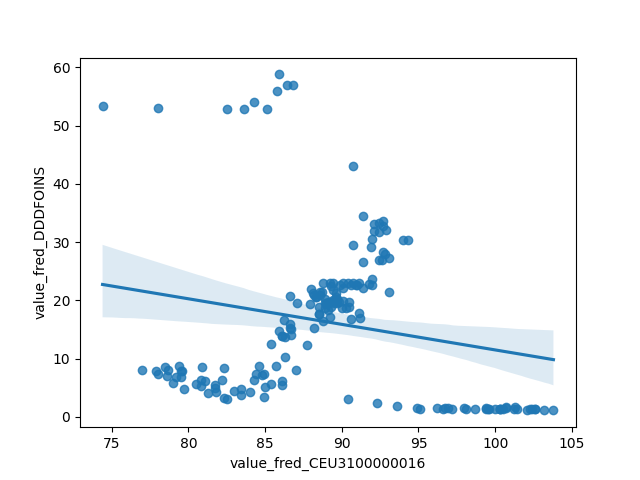
\includegraphics[scale = 0.9]{plots/plot_2026-09-02.png}
\caption{Raw Regression Plot for 2026-09-02}
\end{figure}
\newpage
\subsection{Detrended Regression}
\noindent Regresses the residuals of each series after removing its own linear time trend, so a shared trend can no longer drive the result on its own. A relationship that stays significant here is better evidence of a genuine link between the two series.

\begin{center}
\begin{tabular}{lclc}
\toprule
\textbf{Dep. Variable:}                        & value\_fred\_DDDFOINS\_detrended & \textbf{  R-squared:         } &     0.000   \\
\textbf{Model:}                                &               OLS                & \textbf{  Adj. R-squared:    } &    -0.005   \\
\textbf{Method:}                               &          Least Squares           & \textbf{  F-statistic:       } &   0.05396   \\
\textbf{Date:}                                 &         Wed, 02 Sep 2026         & \textbf{  Prob (F-statistic):} &    0.817    \\
\textbf{Time:}                                 &             15:25:54             & \textbf{  Log-Likelihood:    } &   -568.24   \\
\textbf{No. Observations:}                     &                 179              & \textbf{  AIC:               } &     1140.   \\
\textbf{Df Residuals:}                         &                 177              & \textbf{  BIC:               } &     1147.   \\
\textbf{Df Model:}                             &                   1              & \textbf{                     } &             \\
\textbf{Covariance Type:}                      &            nonrobust             & \textbf{                     } &             \\
\bottomrule
\end{tabular}
\begin{tabular}{lcccccc}
                                               & \textbf{coef} & \textbf{std err} & \textbf{t} & \textbf{P$> |$t$|$} & \textbf{[0.025} & \textbf{0.975]}  \\
\midrule
\textbf{const}                                 &   -1.765e-14  &        0.435     & -4.06e-14  &         1.000        &       -0.858    &        0.858     \\
\textbf{value\_fred\_CEU3100000016\_detrended} &      -0.0165  &        0.071     &    -0.232  &         0.817        &       -0.157    &        0.124     \\
\bottomrule
\end{tabular}
\begin{tabular}{lclc}
\textbf{Omnibus:}       & 69.935 & \textbf{  Durbin-Watson:     } &    0.069  \\
\textbf{Prob(Omnibus):} &  0.000 & \textbf{  Jarque-Bera (JB):  } &  182.593  \\
\textbf{Skew:}          &  1.695 & \textbf{  Prob(JB):          } & 2.24e-40  \\
\textbf{Kurtosis:}      &  6.605 & \textbf{  Cond. No.          } &     6.13  \\
\bottomrule
\end{tabular}
%\caption{OLS Regression Results}
\end{center}

Notes: \newline
 [1] Standard Errors assume that the covariance matrix of the errors is correctly specified.

\begin{figure}
\centering
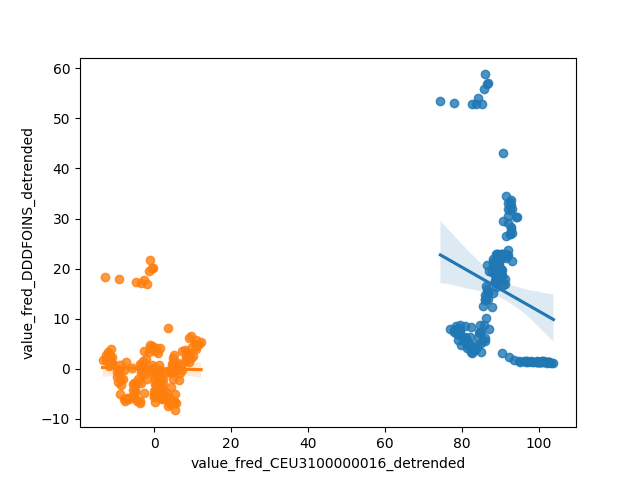
\includegraphics[scale = 0.9]{plots/plot_2026-09-02_detrended.png}
\caption{Detrended Regression Plot for 2026-09-02}
\end{figure}
\newpage
